\documentclass{article}
\usepackage[utf8]{inputenc}
\usepackage{amssymb,amsmath}
\usepackage[parfill]{parskip}
\DeclareMathOperator*{\argmin}{arg\,min}
\DeclareMathOperator*{\argmax}{arg\,max}
\usepackage{graphicx}
\usepackage{subcaption}

\usepackage{mathtools}
\DeclareMathOperator{\tr}{tr}

\title{Optimization 10/36-725\\
        Homework 2}
\author{Willie Neiswanger}
\date{}

\begin{document}

\maketitle


\section{Problem Five}

\begin{figure}[h!tbp]
        \center{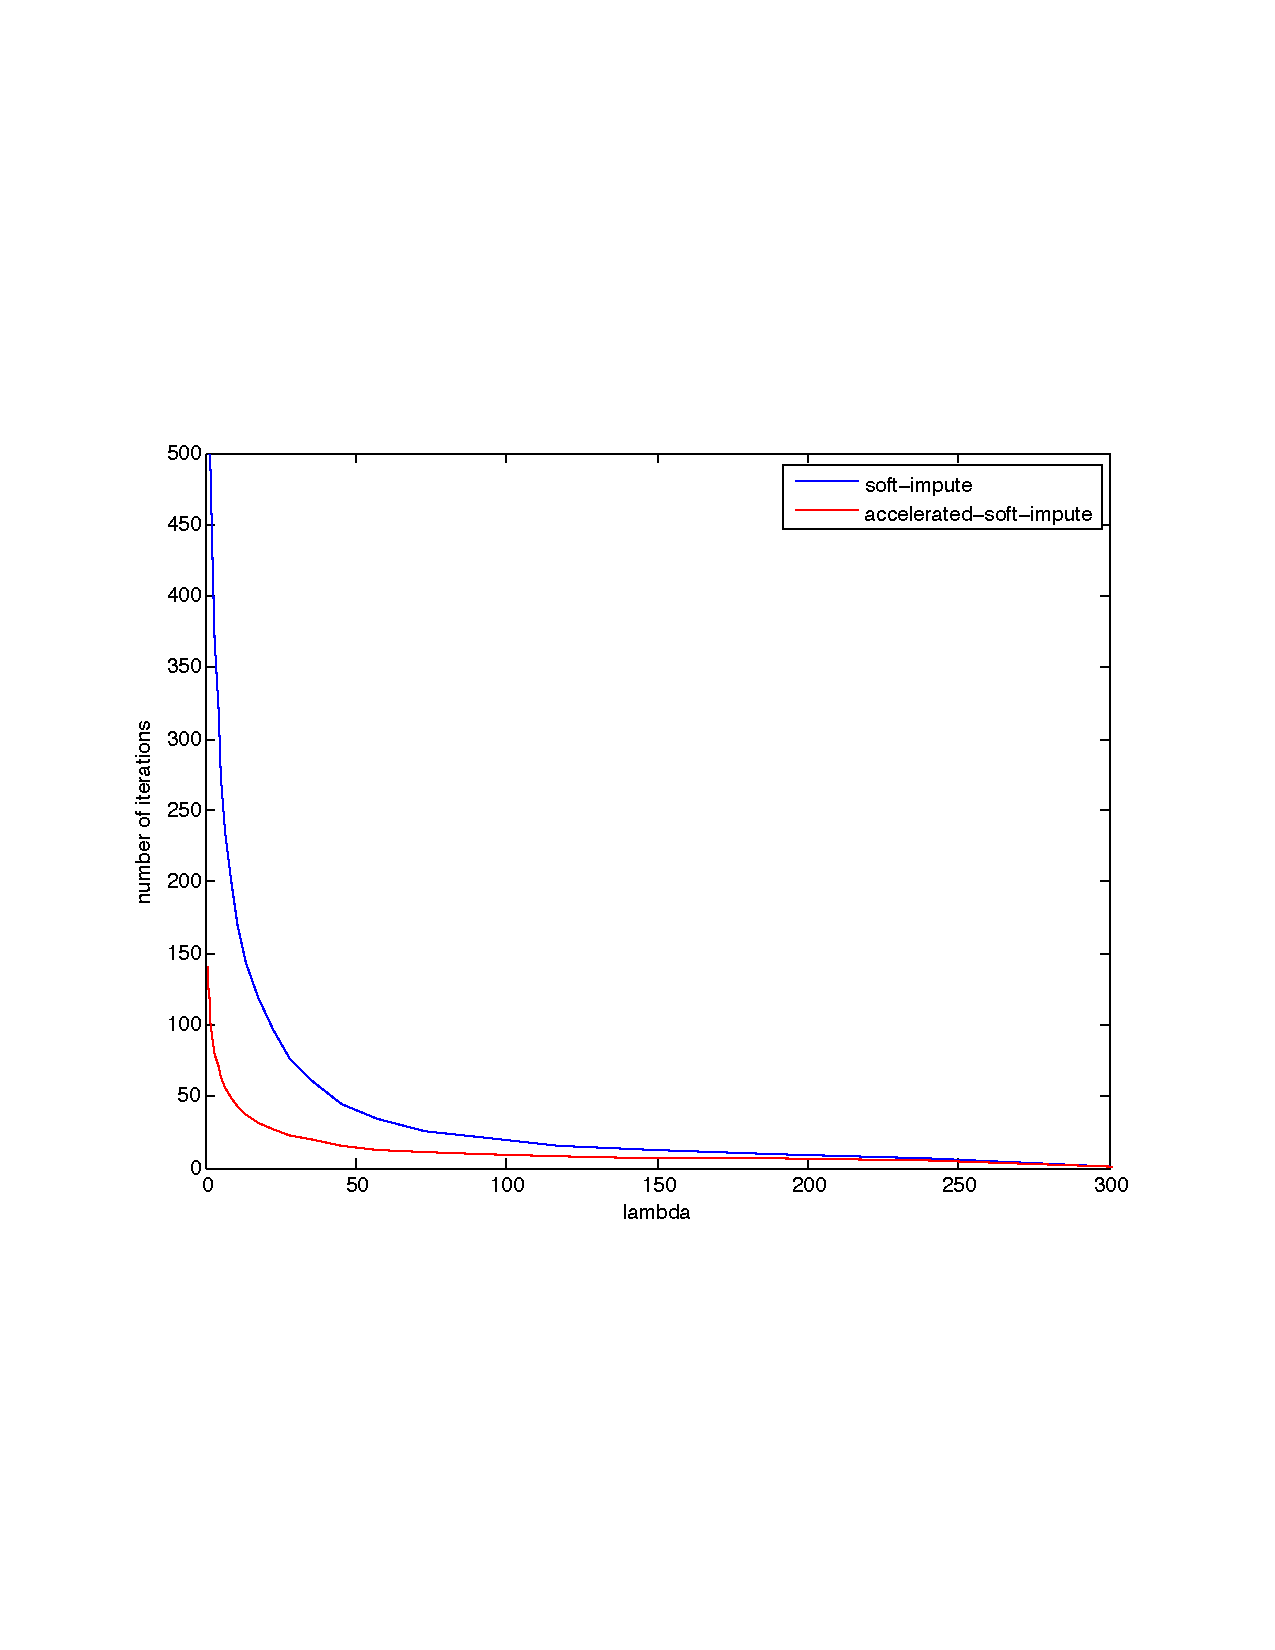
\includegraphics[width=0.7\textwidth]{img/p5_01.pdf}}
        \caption{This plot shows the number of iterations until convergence vs
        the lambda value for both the accelerated and non-accelerated soft-impute
        algorithm. It appears that acceleration allows for quicker convergence
        to the optimal value here, as the accelerated algorithm never needs
        the full 500 iterations.}
\end{figure}

\begin{figure}[h!tbp]
        \center{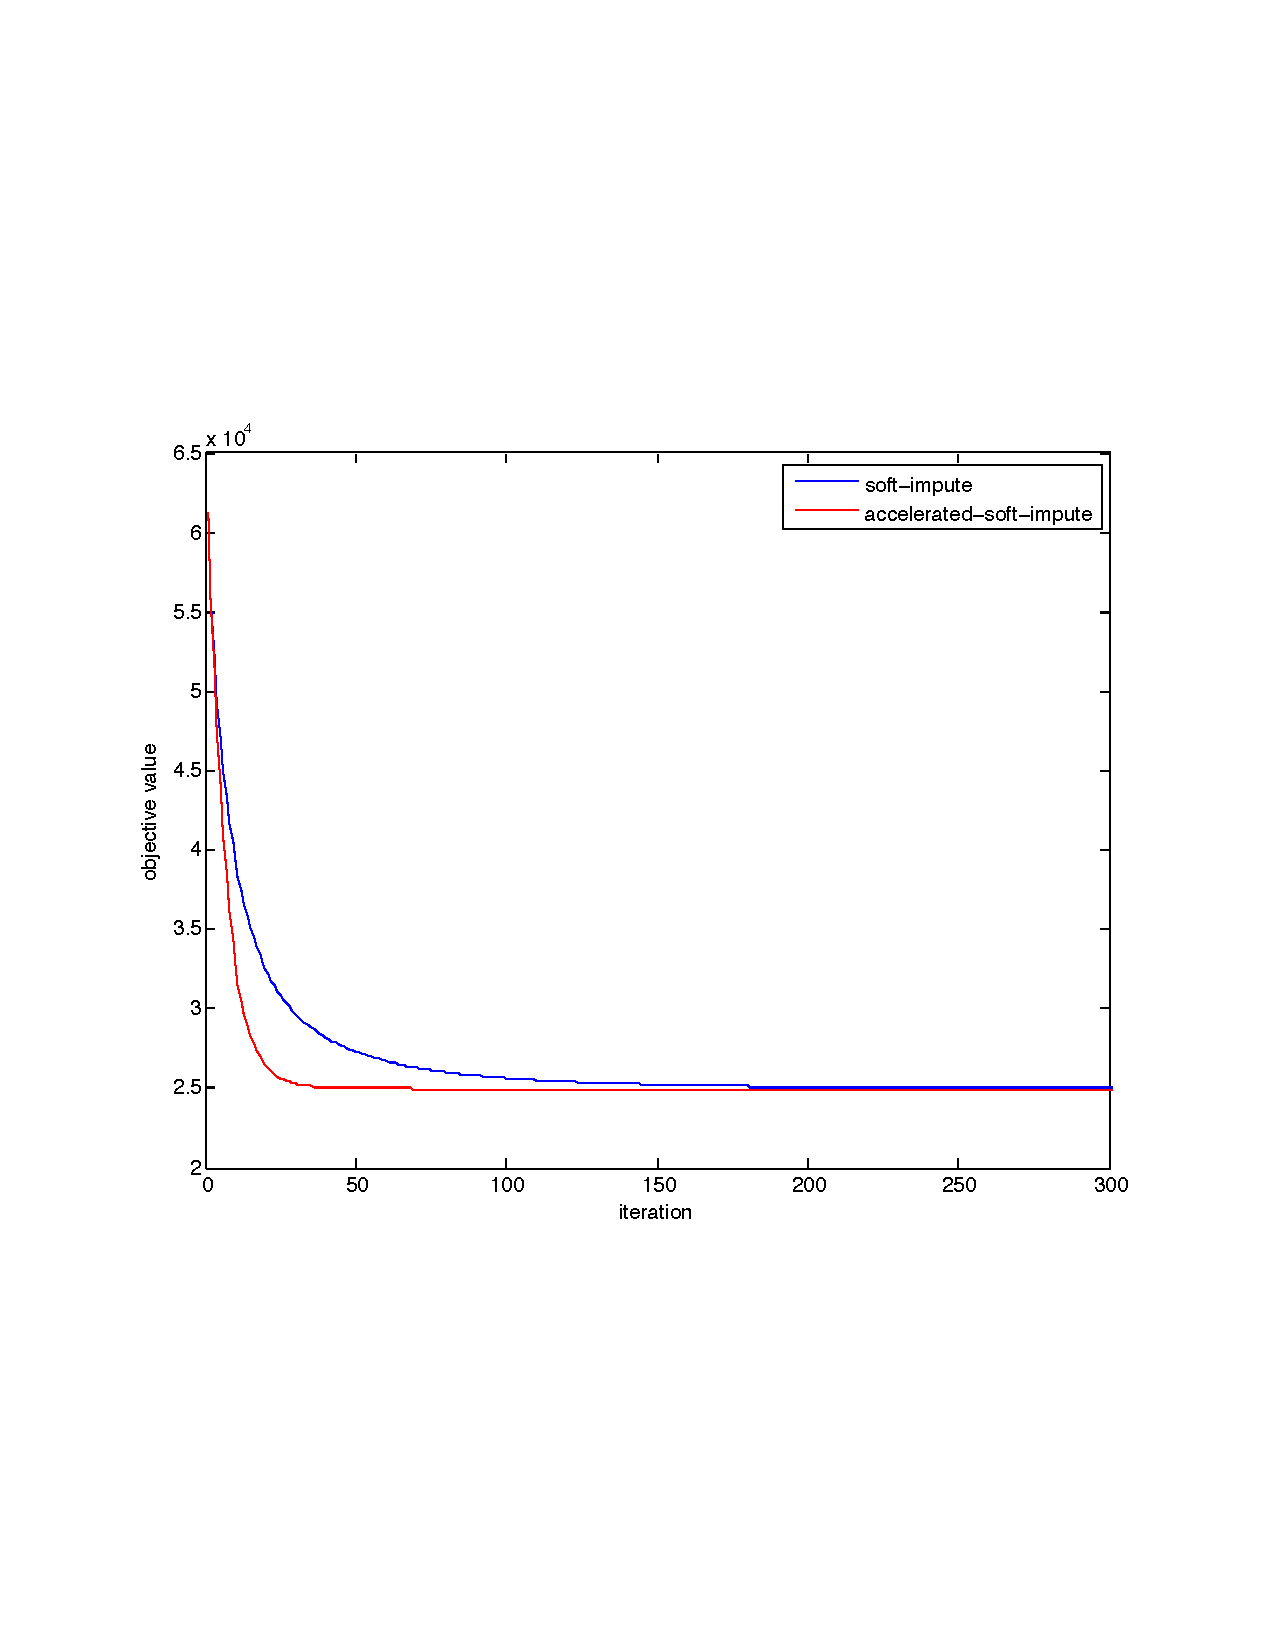
\includegraphics[width=0.7\textwidth]{img/p5_02.pdf}}
        \caption{This plot shows the objective value vs iteration number for
        both the accelerated and non-accelerated soft-impute algorithms (for a
        fixed lamba=10). Both algorithms converge to a small, similar objective
        value, though the accelerated algorithm converges more quickly.}
\end{figure}

\begin{figure}[h!tbp]
    \centering
    \begin{subfigure}[a]{0.3\textwidth}
        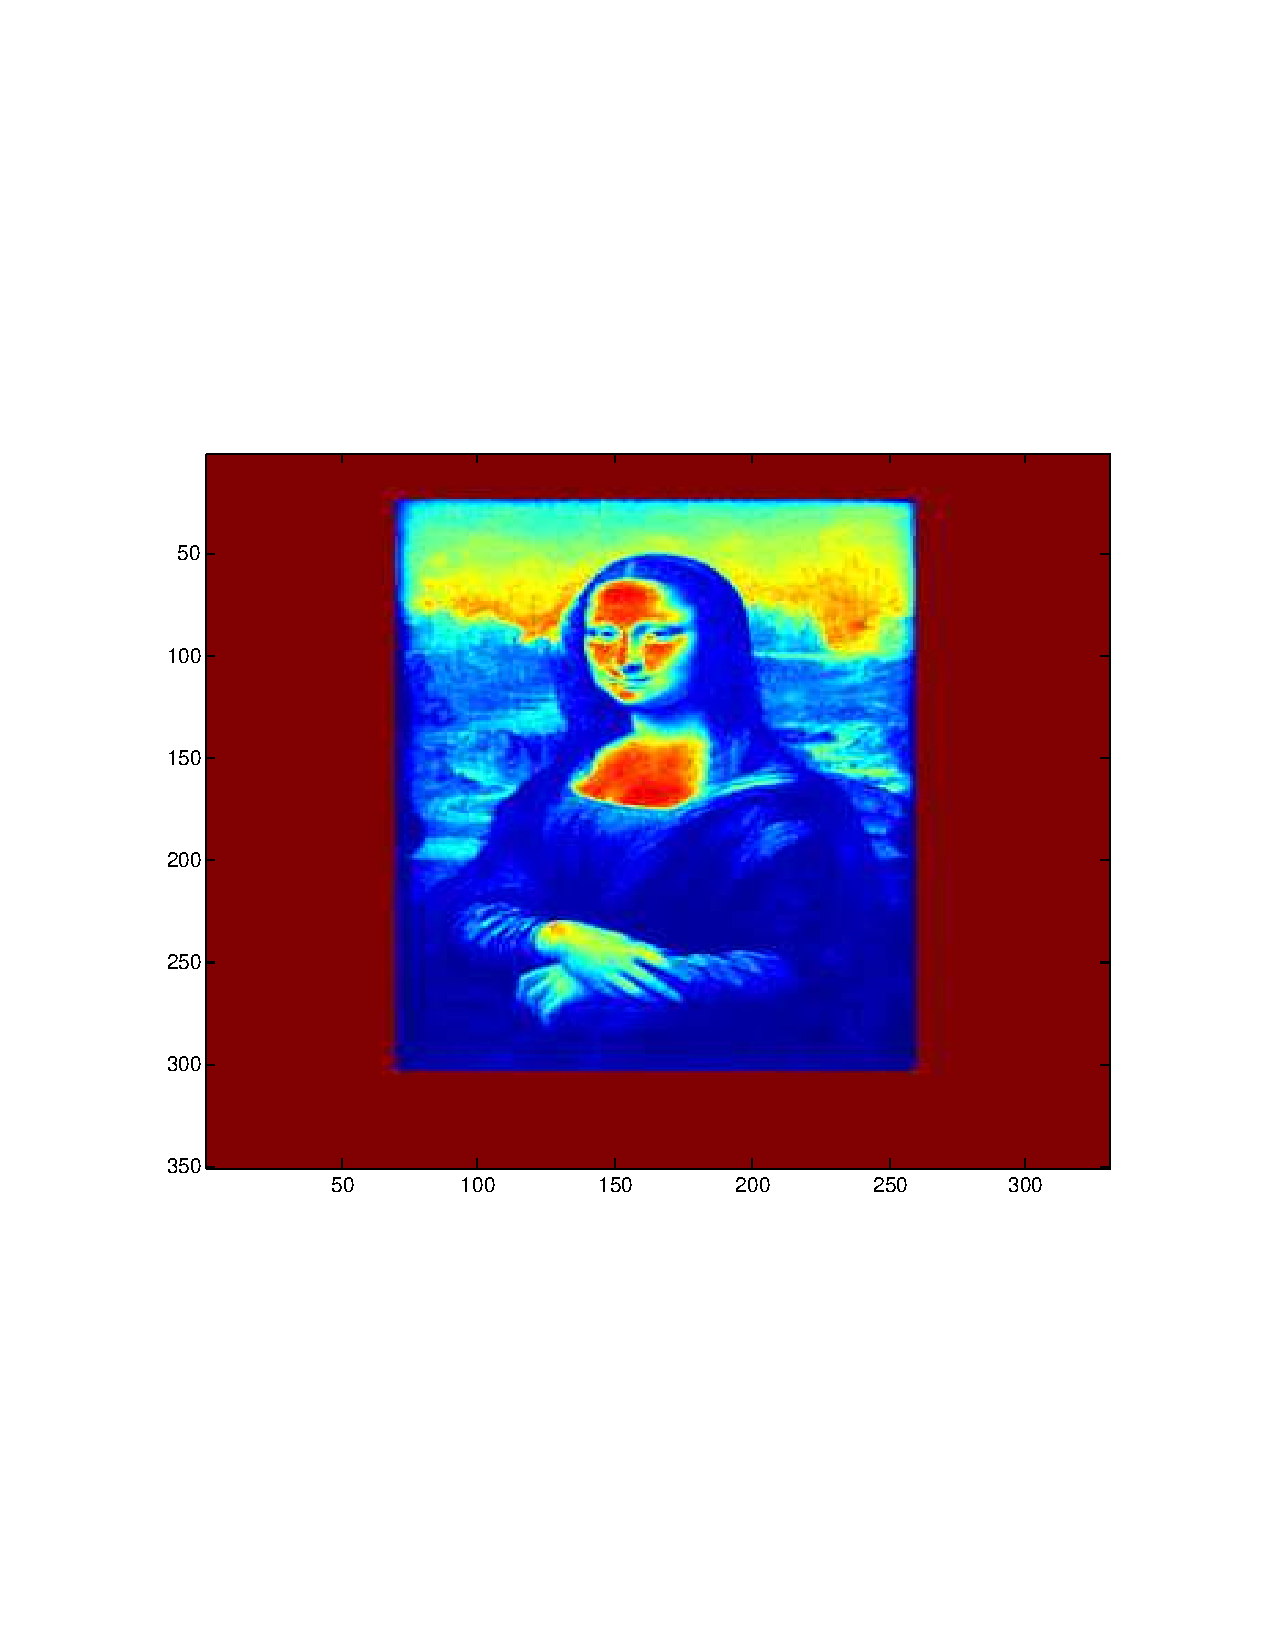
\includegraphics[width=\textwidth]{img/p5_mona.pdf}
    \end{subfigure}
    \begin{subfigure}[a]{0.3\textwidth}
        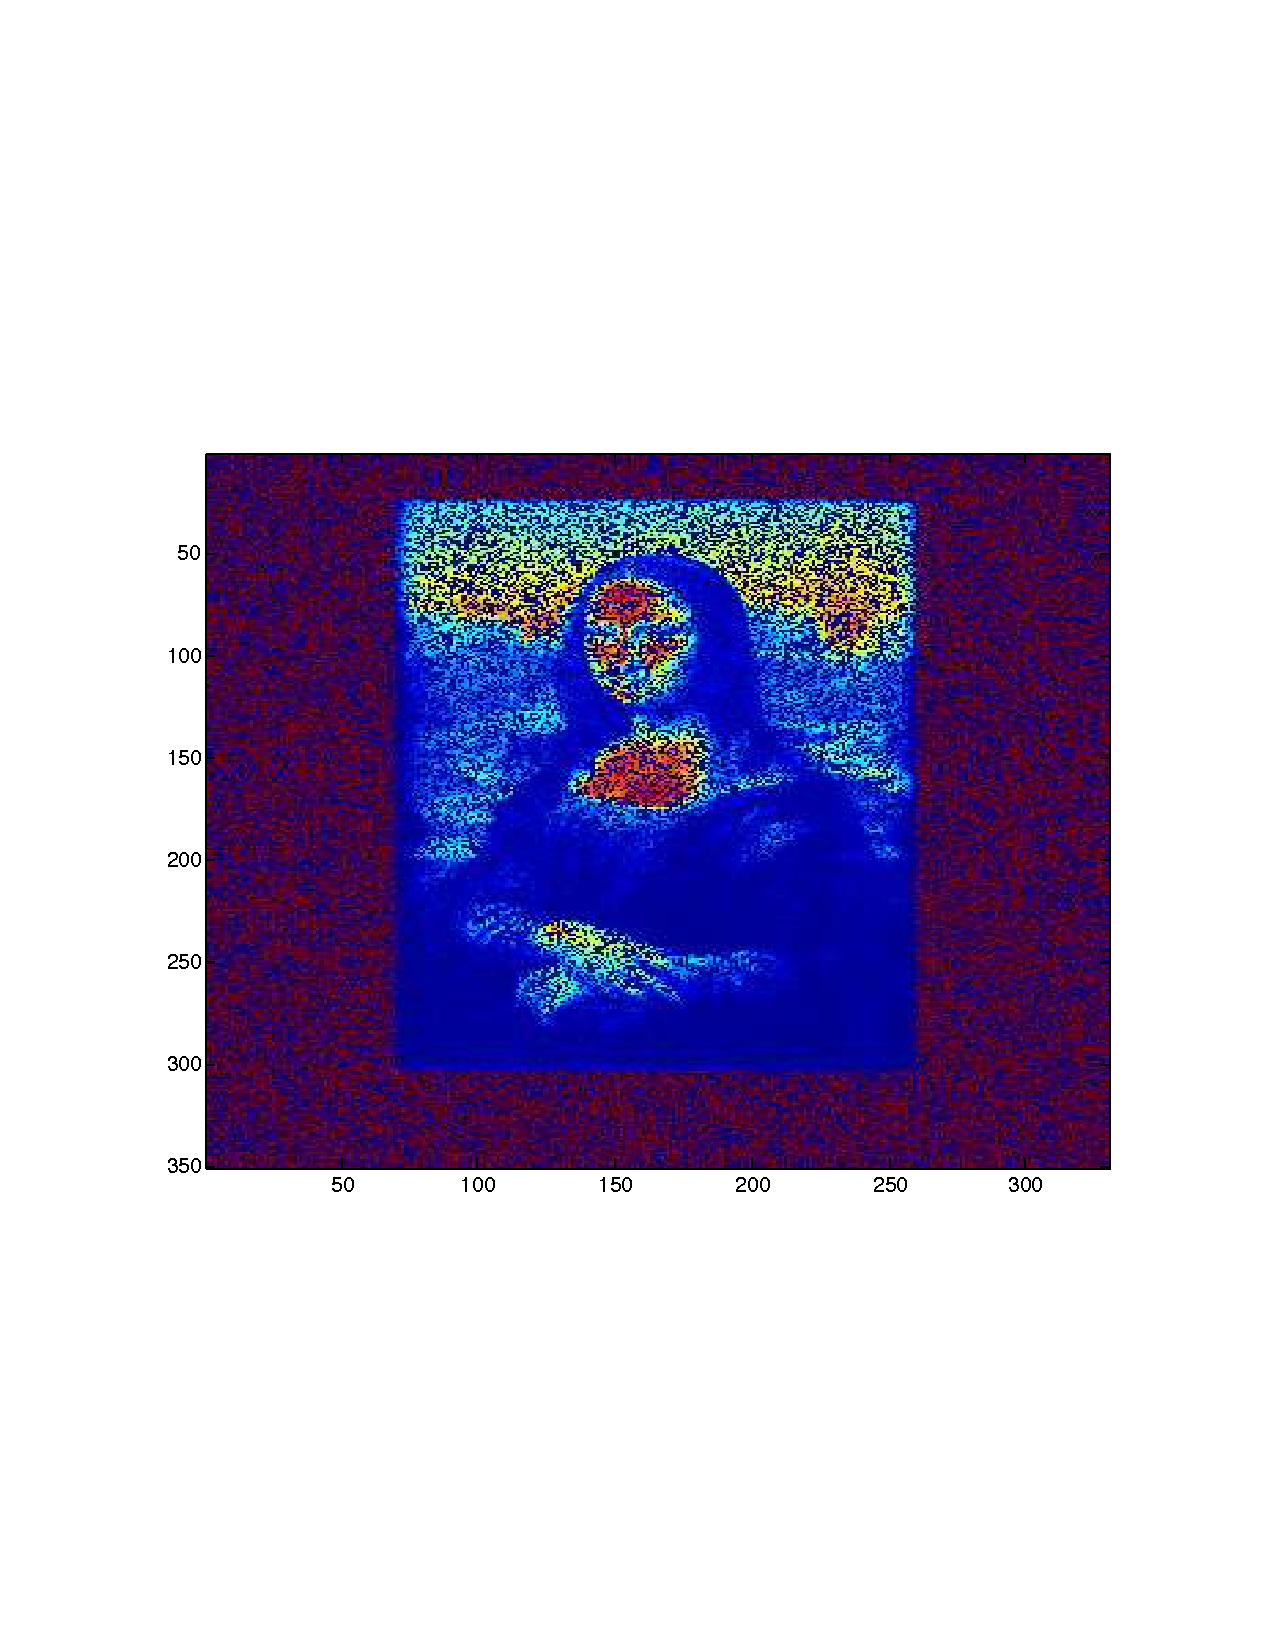
\includegraphics[width=\textwidth]{img/p5_mona1.pdf}
    \end{subfigure}
    \begin{subfigure}[a]{0.3\textwidth}
        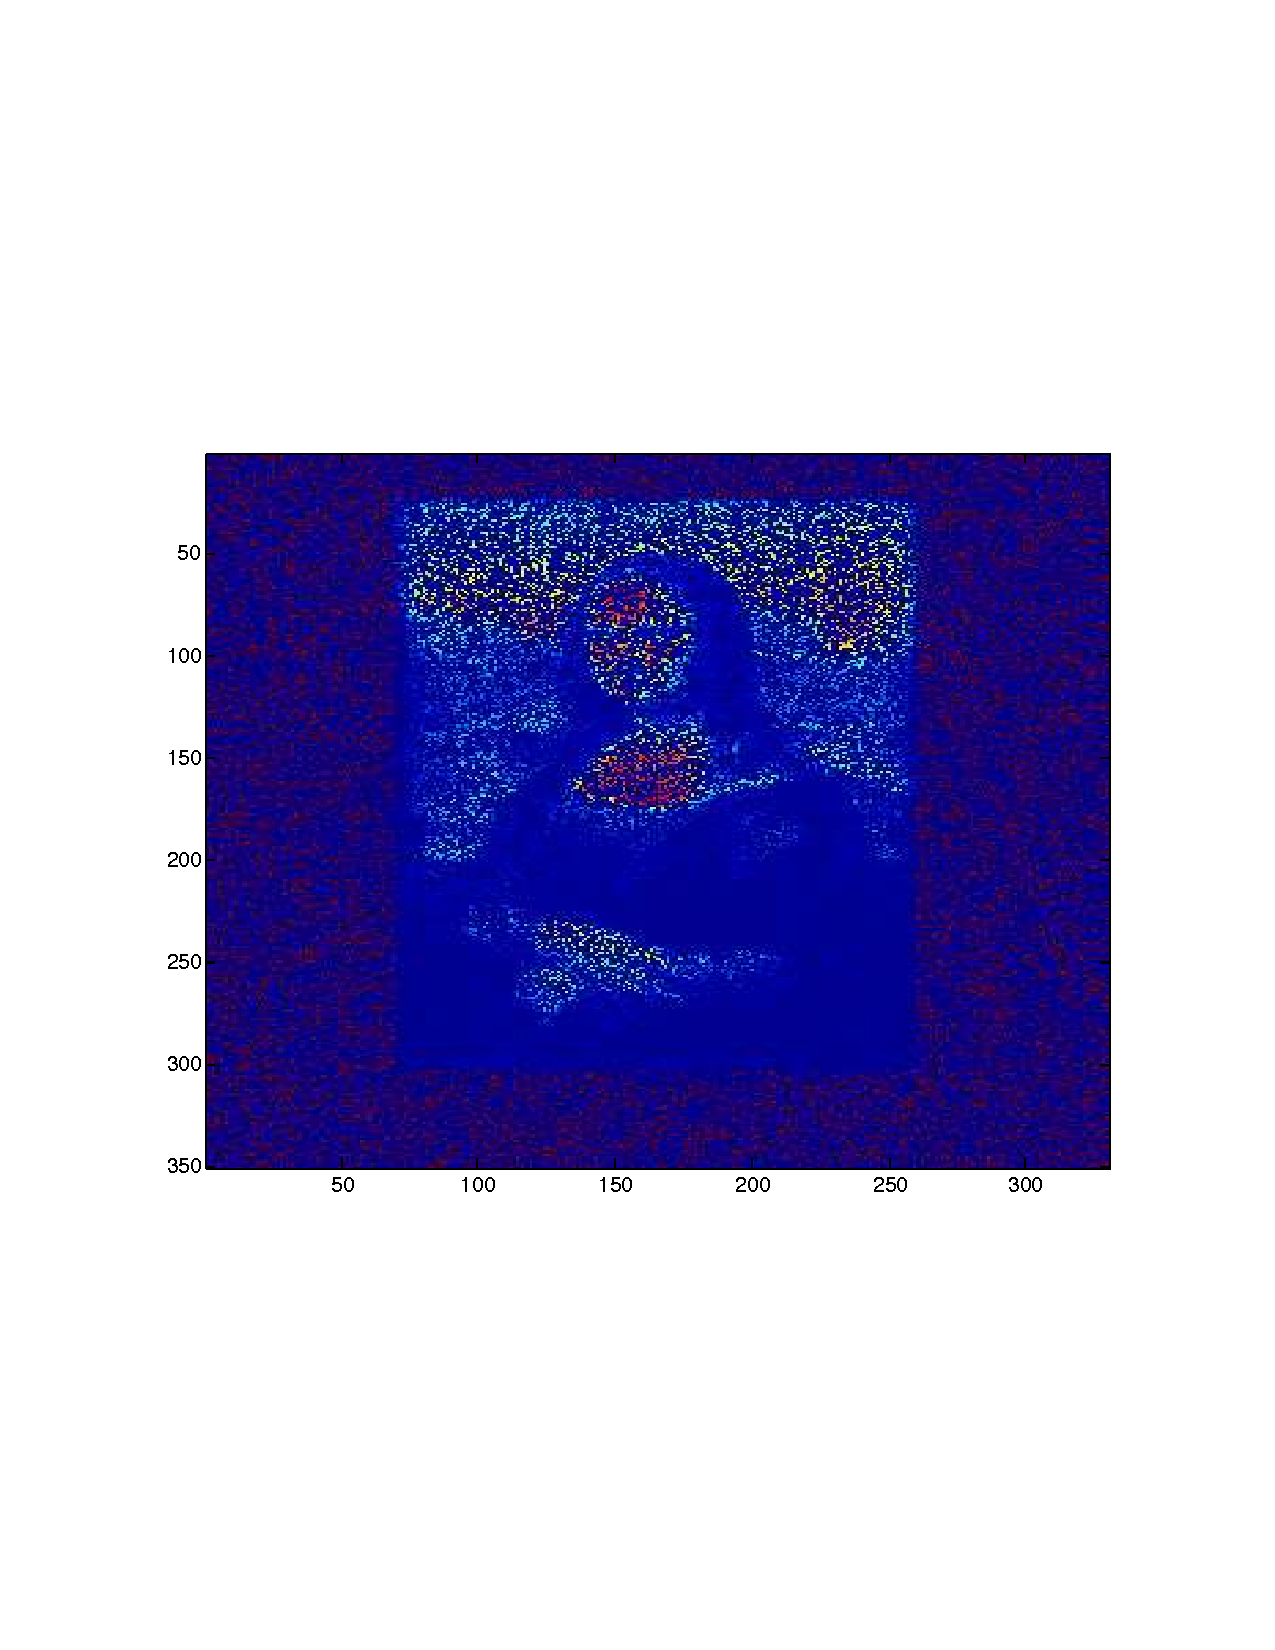
\includegraphics[width=\textwidth]{img/p5_mona2.pdf}
    \end{subfigure}
    \caption{This plot shows the initial Mona Lisa image, and the same image subsampled at $50\%$ and $20\%$.} 
\end{figure}

\begin{figure}[h!tbp]
    \centering
    \begin{subfigure}[a]{0.3\textwidth}
        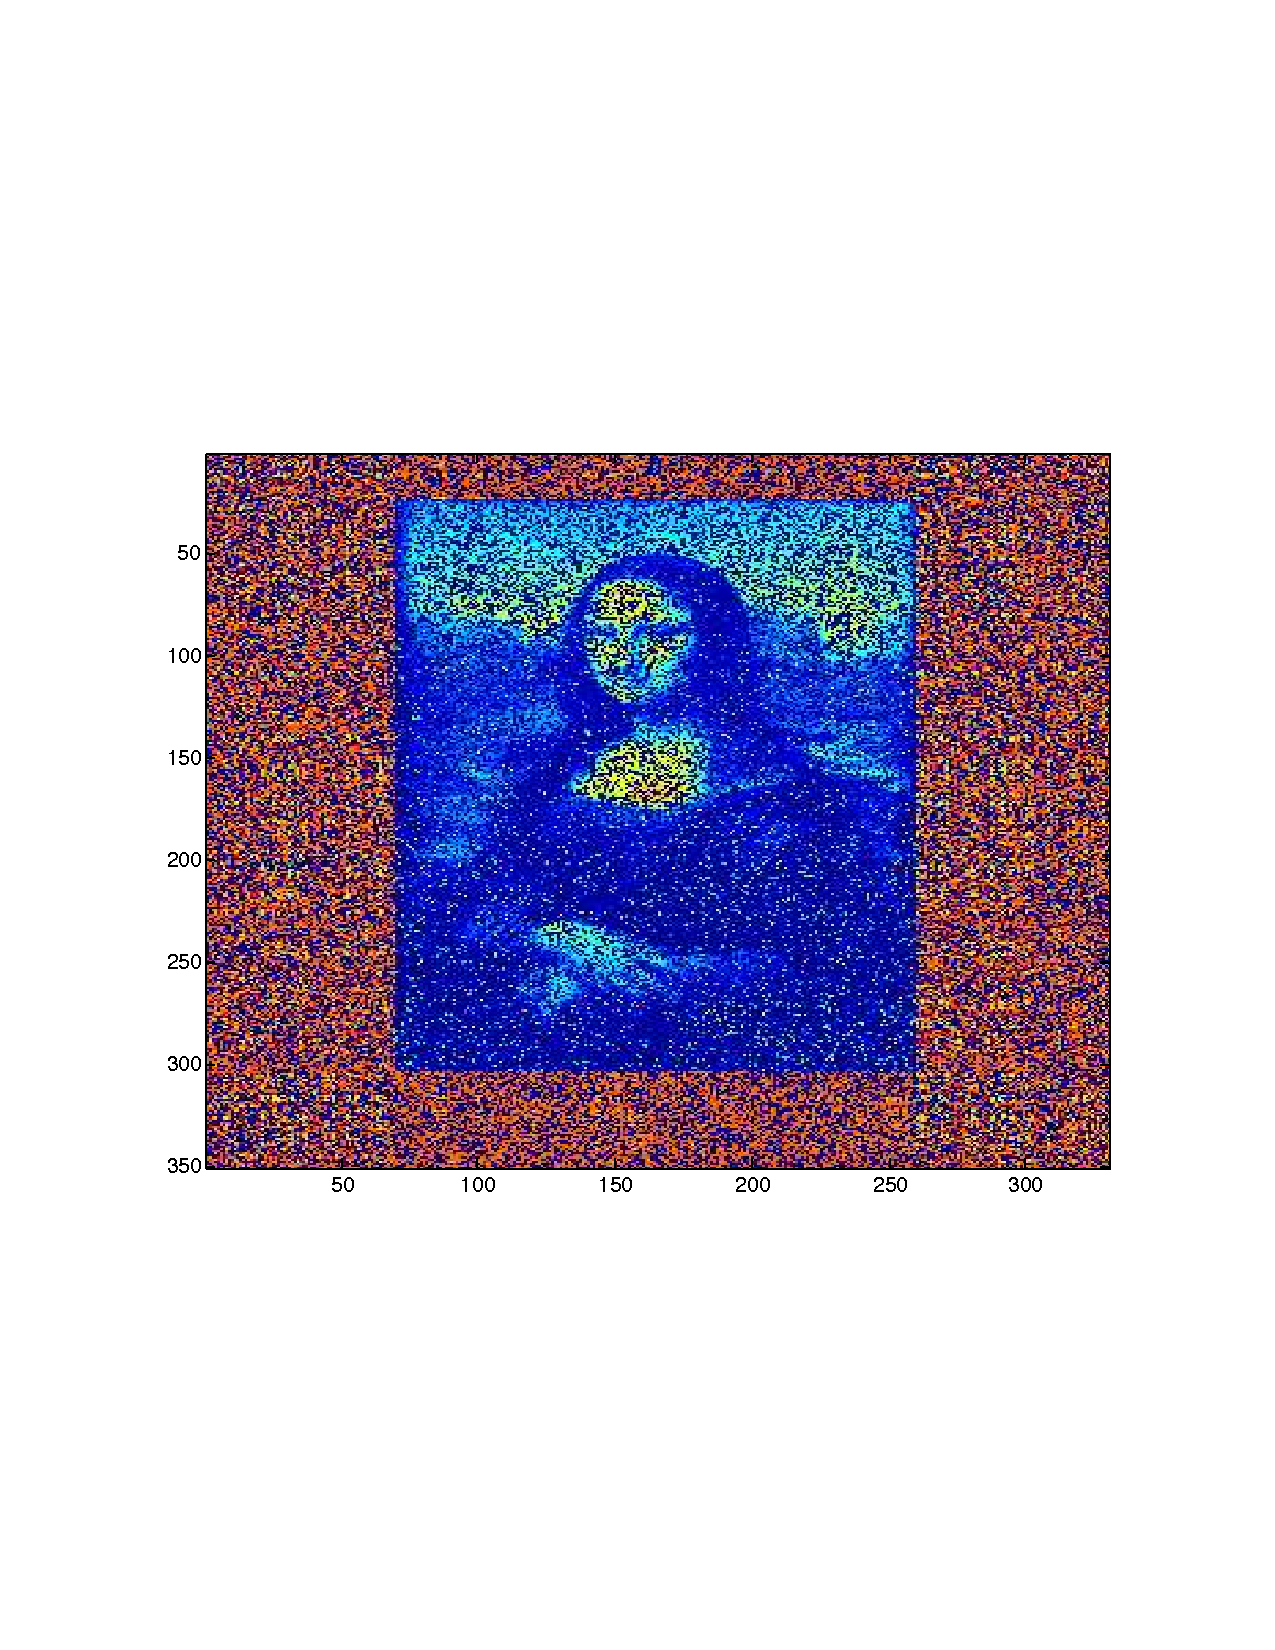
\includegraphics[width=\textwidth]{img/p5_m1_lam1.pdf}
    \end{subfigure}
    \begin{subfigure}[b]{0.3\textwidth}
        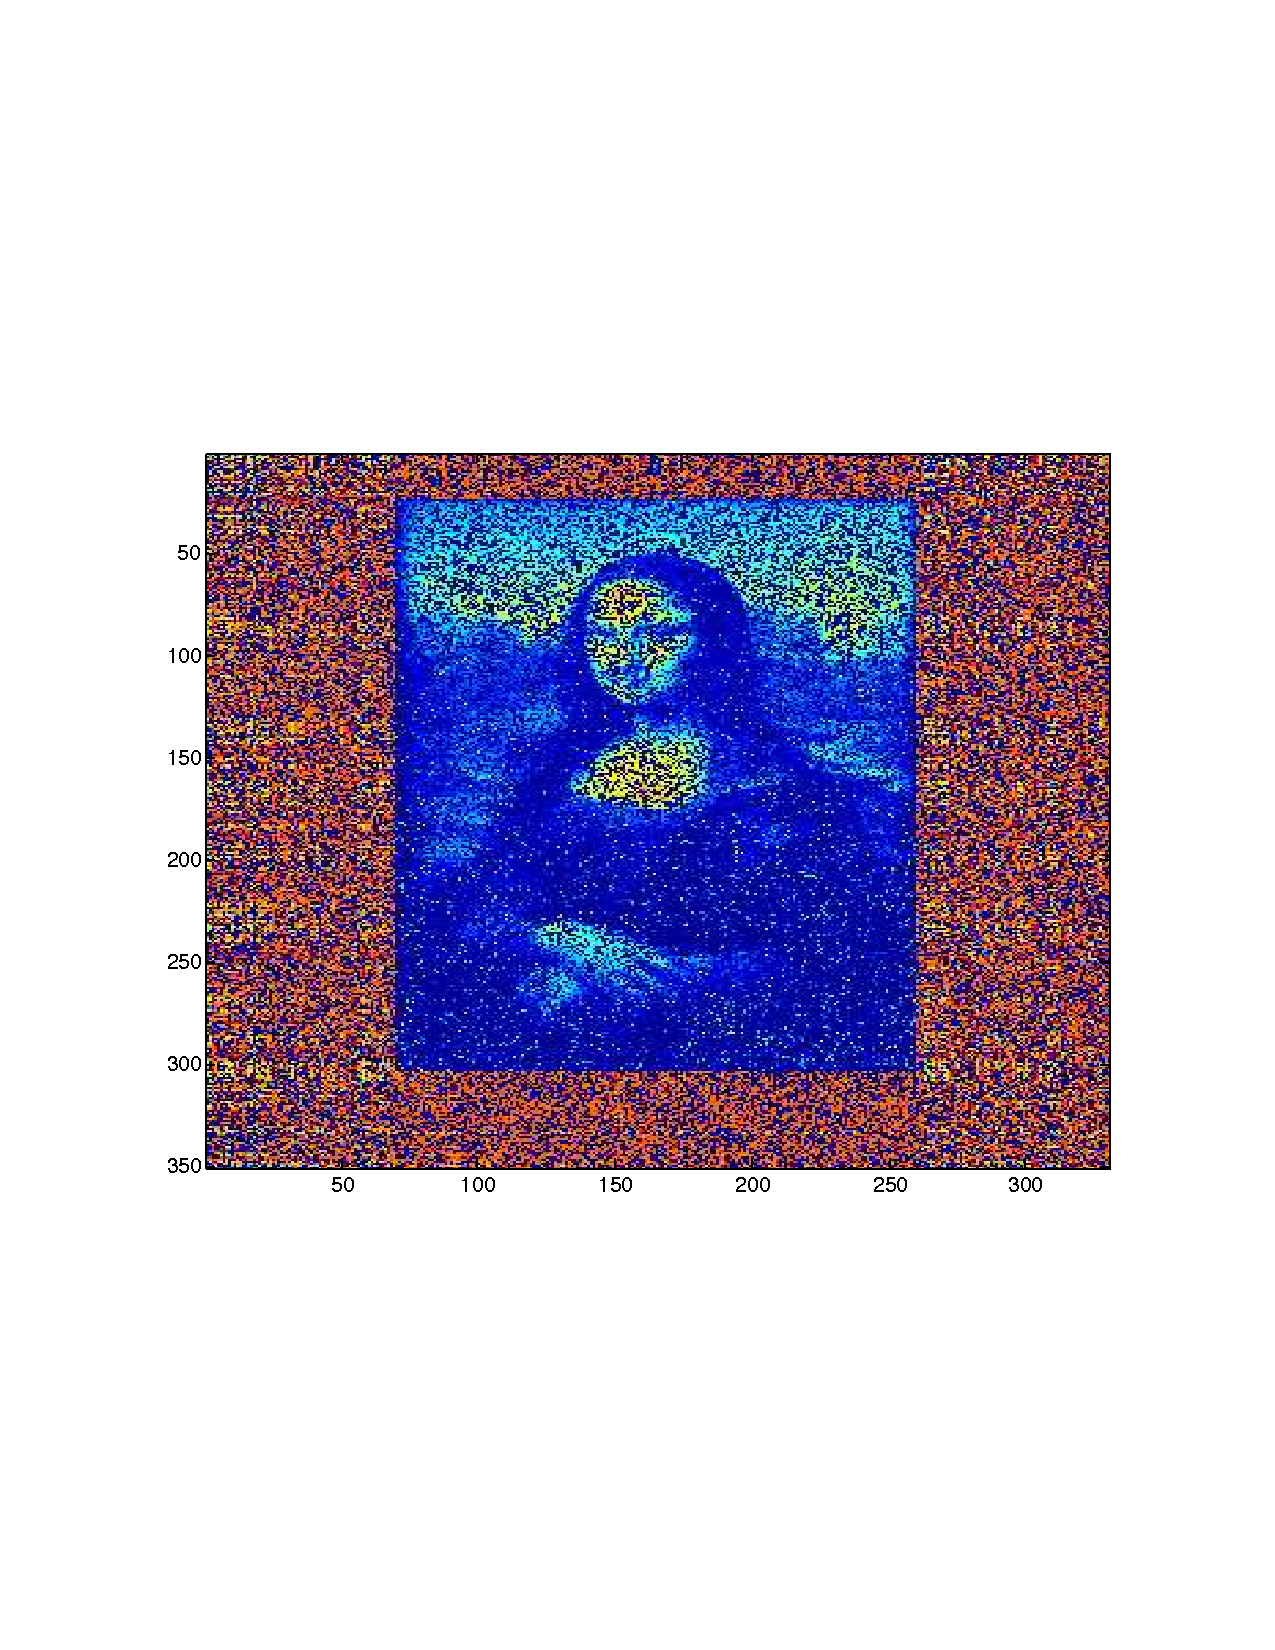
\includegraphics[width=\textwidth]{img/p5_m1_lam2.pdf}
    \end{subfigure}
    \begin{subfigure}[c]{0.3\textwidth}
        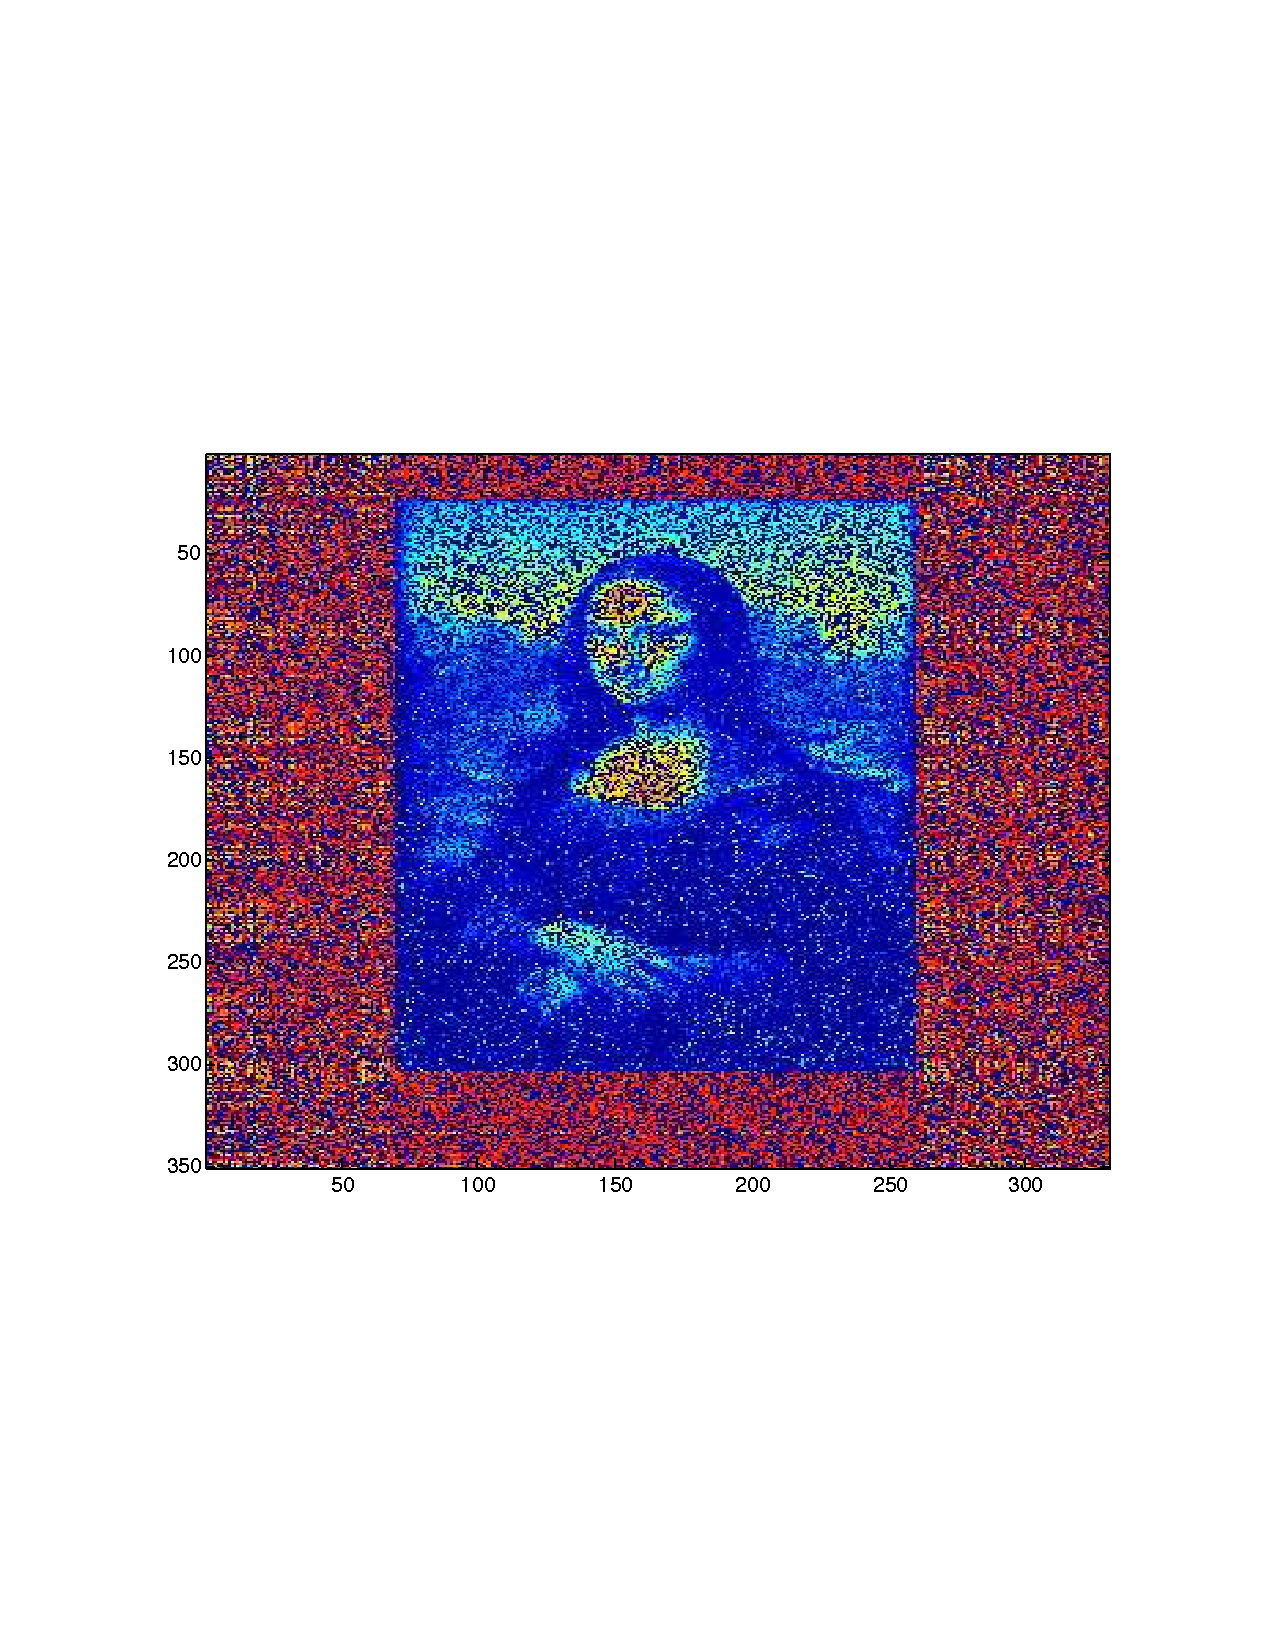
\includegraphics[width=\textwidth]{img/p5_m1_lam3.pdf}
    \end{subfigure}
    \begin{subfigure}[d]{0.3\textwidth}
        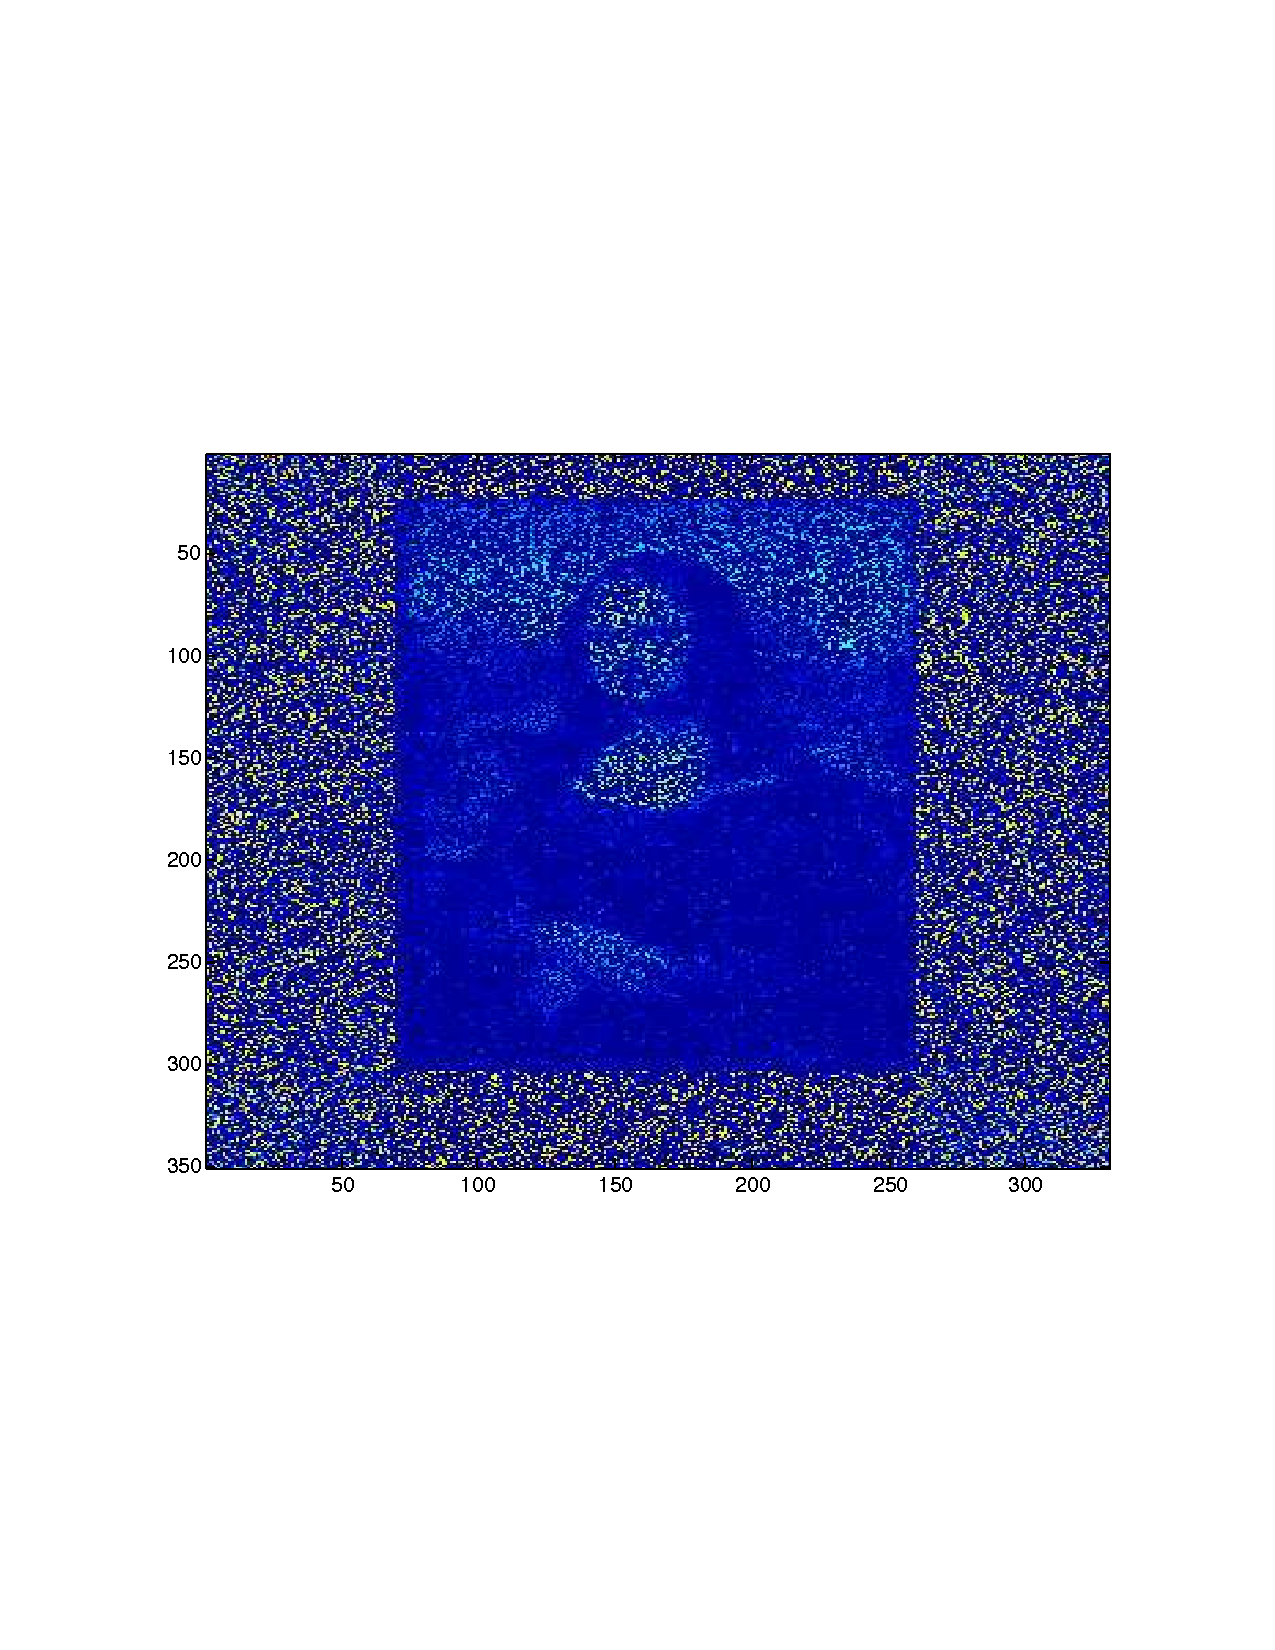
\includegraphics[width=\textwidth]{img/p5_m2_lam1.pdf}
    \end{subfigure}
    \begin{subfigure}[e]{0.3\textwidth}
        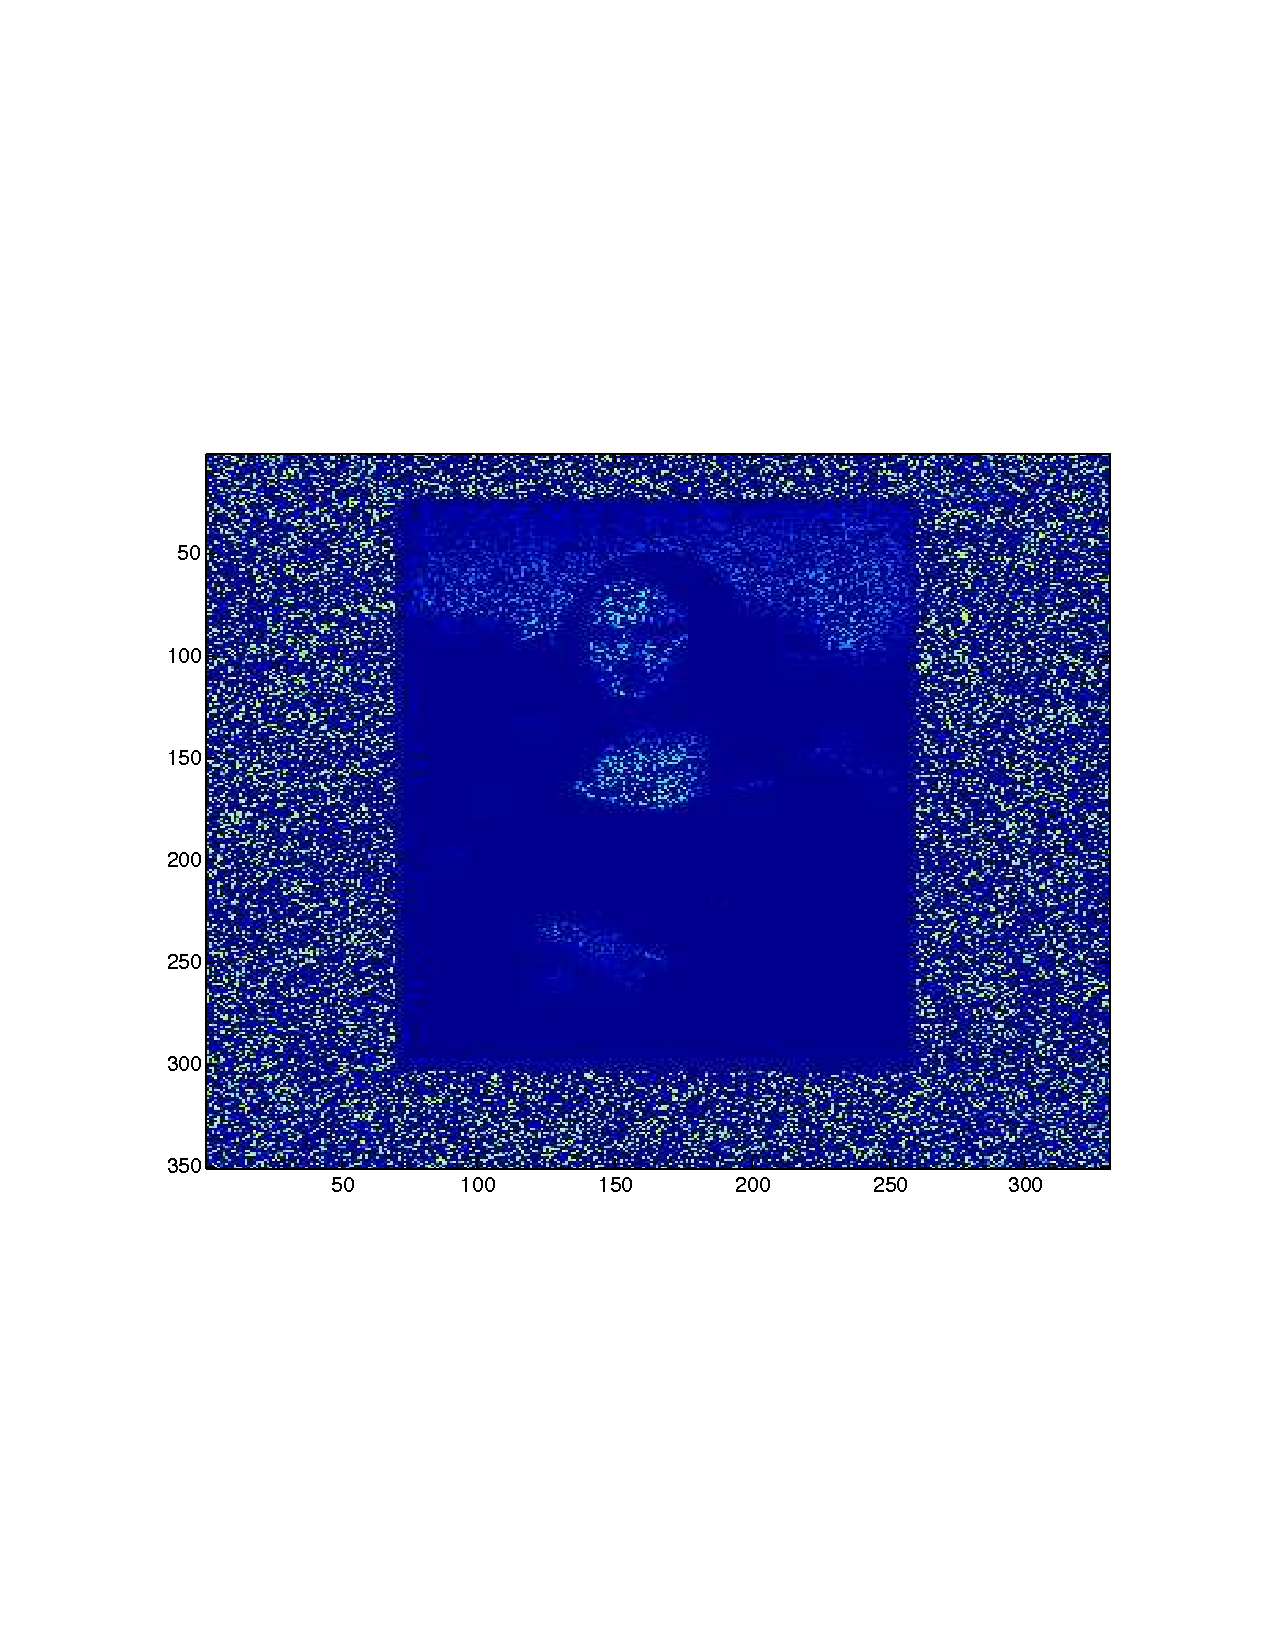
\includegraphics[width=\textwidth]{img/p5_m2_lam2.pdf}
    \end{subfigure}
    \begin{subfigure}[f]{0.3\textwidth}
        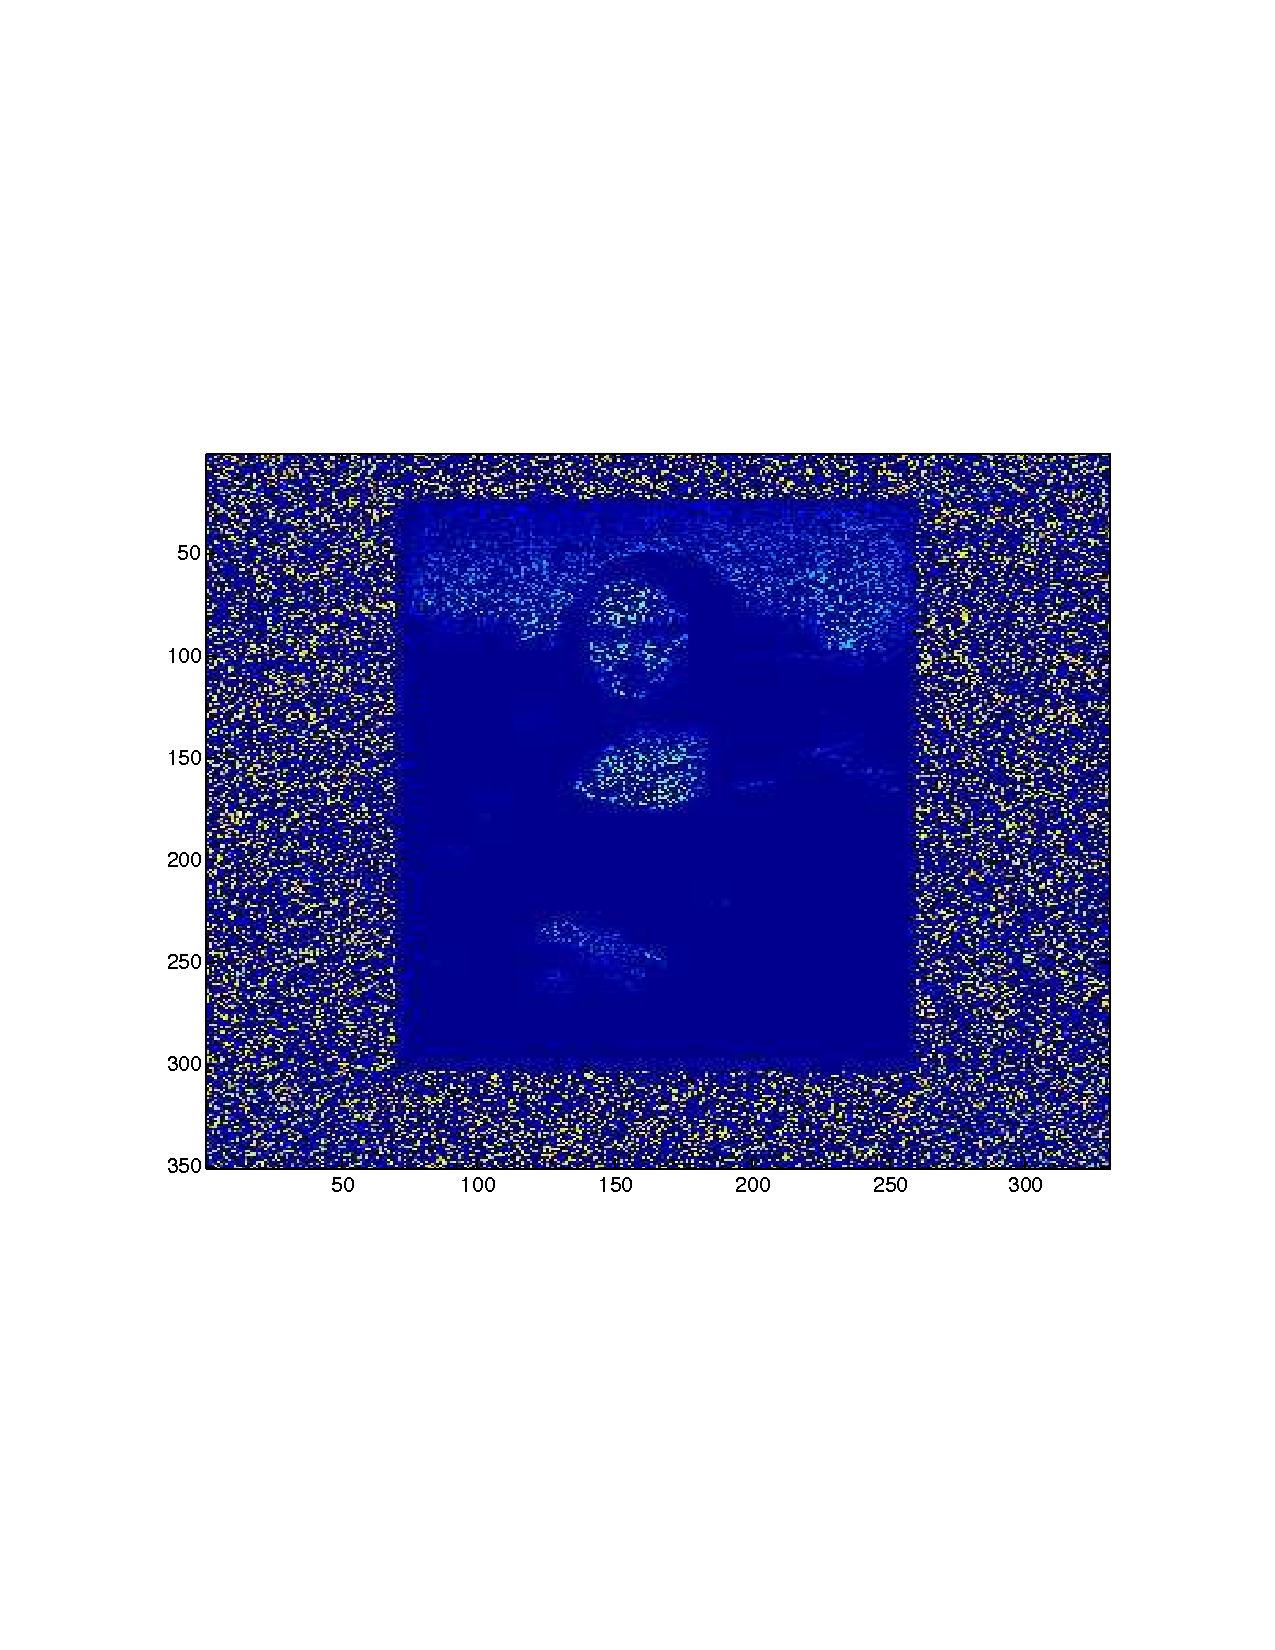
\includegraphics[width=\textwidth]{img/p5_m2_lam3.pdf}
    \end{subfigure}
    \caption{This plot shows the reconstructed Mona Lisa images for three
    lambda values (10, 50, and 100), for both $50\%$ subsampling (top row) and
    $20\%$ subsampling (bottom row). It appears that a lambda value of 10
    yielded the best value for the $50\%$ subsampling and a lambda of 50
    yielded the best value for the $20\%$ subsampling (so a higher value was
    better as the subsampling decreased).} 
\end{figure}


\end{document}
